\section{亚线性复杂度PIR基础协议}
本文设计的可验证PIR基于现有的亚线性PIR协议\cite{EC:CorKog20, C:LazPap23}。我们从如图\ref{fig:CK20}所示的两服务器PIR基础协议起步,分析其中的问题,讨论如何修正该基础协议的局限性。该协议是一个离线-在线PIR协议,我们使用$\hintserver$ 与 $\queryserver$ 两个记号来区分协议中涉及到的两台服务器。这些记号是根据两台服务器的功能定义的,其中$\hintserver$负责处理Hint请求,而$\queryserver$处理真正的查询:

\subsection{基础协议}

\noindent \textbf{离线阶段:}
\begin{itemize}
\item \textbf{Setup:} 客户端$\client$ 生成$\hintcount$ 组集合$\setkey_j, j\in[\hintcount]$。每个集合包含$\setsize$个在范围[$\dbsize$]内的随机索引。
\item \textbf{Hint:} $\client$将这些集合转发给$Hint$服务器$\hintserver$。$\hintserver$计算这些集合对应数据库中记录的和,表示为$\hint_j \coloneqq \sum_{k\in \setkey_j} \db_k, j \in [\hintcount]$。$\client$存储这些集合及其对应的记录之和作为校验值。
\end{itemize}

\noindent \textbf{在线阶段:}
\begin{itemize}
\item \textbf{Query:} $\client$首先找出一个包含目标索引$\dbidx$的集合$\setkey_\hintidx$,并从该集合中去掉$\dbidx$,$\queryquery \coloneqq \setkey_\hintidx \setminus \{\dbidx\}$。此外,$\client$生成一个包含索引$\dbidx$的新集合$\setkey'$,并令$\hintquery \coloneqq \setkey' \setminus \{\dbidx\}$。$\client$将集合$\hintquery$发送给$Hint$服务器$\hintserver$,将$\queryquery$发送给$Query$服务器$\queryserver$。
\item \textbf{Answer:} 收到这些集合后,服务器分别为两个集合计算校验值,$\queryanswer\coloneqq \sum_{j\in \queryquery}\db_j$,$\hintanswer\coloneqq \sum_{j\in \hintquery}\db_j$,将这些校验值发送给$\client$。
\item \textbf{Reconstruct:} $\client$ 计算出所需的记录:$\db_\dbidx \coloneqq \hint_\hintidx - \queryanswer$。
\item \textbf{Refresh:} $\client$ 更新$Hint$: $\setkey_\hintidx \coloneqq \setkey'$,$\hint_\hintidx \coloneqq \hintanswer+\db_\dbidx$。
\end{itemize}


\subsection{基础协议的缺陷}
不妨先假设客户端生成的集合足够多,多到在$Query$阶段能以足够大的概率找到包含目标索引的集合。在此前提下,客户端总能得到想要查询的记录$\db_\dbidx$,这使得该协议的正确性得到保证。然而,该协议存在三个关键问题:

\begin{enumerate}
\item \textbf{低效的集合隶属测试:} 搜索包含查询索引$\dbidx$的集合$\setkey_t$的过程计算量很大。客户端需要遍历所有集合,同时枚举集合中的元素以确定某个索引是否隶属于这个集合。尽管可以通过排序和二分查找优化在集合内枚举的过程,但一次搜索仍然需要$O(\sqrt{\dbsize}\log \dbsize)$的在线计算复杂度。
\item \textbf{低下的空间和通信效率:} 以明文形式生成、存储和发送这些集合的效率很低,粗略估计,为了确保正确性,客户端需要大约$\hintcount = O(\lambda\sqrt{\dbsize})$个集合,每个集合的大小为$\setsize = \sqrt{\dbsize}$。相应的存储和离线通信复杂度为$O(\lambda\dbsize)$。
\item \textbf{有缺陷的隐私性:} 集合$\queryquery$和$\hintquery$中均不会包含查询的索引$\dbidx$。从信息论角度来看,“必然不包含$\dbidx$”这一事实泄露了大约$1/(\sqrt{\dbsize}\ln 2)$比特$\dbidx$的信息。
\end{enumerate}

\subsection{“虚设查询”及其引入的新问题}
在现有工作中,研究者已经提出了多种方法来解决上述问题。例如,TreePIR \cite{C:LazPap23} 利用了一种称为弱可穿孔伪随机函数(Weakly Puncturable Pseudorandom Function)的原语,并引入了一种新的亚线性PIR协议设计。 Piano \cite{Piano} 提出了一个类似的算法,称为$PossibleParities$。然而,当尝试向这些协议中引入可验证性时,这些方法遇到了类似的困境,本文总结为“虚设查询”。

\begin{figure}
    \centering
    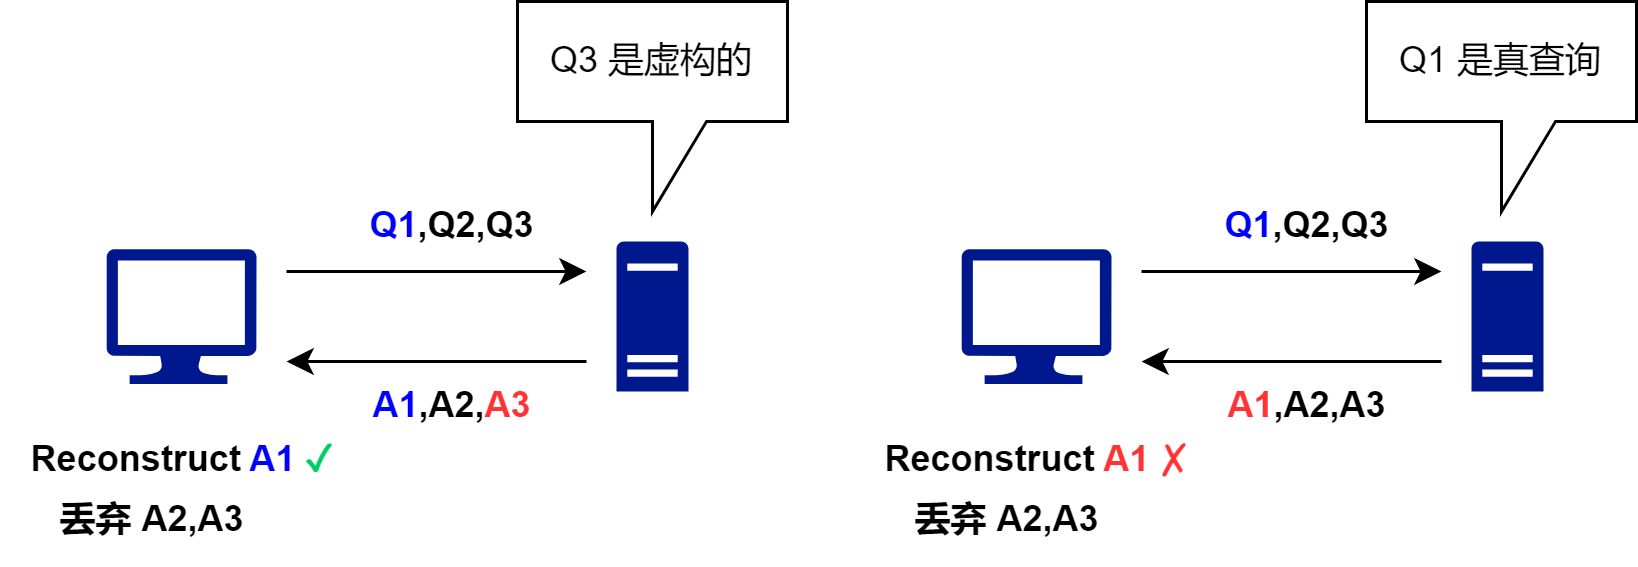
\includegraphics[width=1\linewidth]{figure/dummy.png}
    \caption{关于“虚设查询”的图示}
    \label{fig:dummy}
\end{figure}

这些“虚设查询”是随机生成的假查询,其目的是与真实查询相混淆。在这些协议中,客户端发送的单个查询会泄露关于查询索引$\dbidx$的信息。为解决这一问题,客户端会在一次查询时发送多个请求给服务器,将真实查询混入“虚设查询”中,从而隐藏索引$\dbidx$。服务器无法区分“虚设查询”与真实查询,所以必须对所有查询作出回应,但客户端会忽略对“虚设查询”的回应。

在半诚实环境下,这些协议的隐私性要求服务器无法区分真实查询和“虚设查询”。然而,在可验证PIR的模型中,“选择失败攻击”会使“虚设查询”失效。在验证过程中,由于客户端没有在离线阶段获得这些“虚设查询”的校验信息,因此无法计算和验证“虚设查询”的答案,只能忽略它们。于是,无论一轮查询中“虚设查询”的答案是否正确,只要真实查询的答案通过了验证,客户端都会接受。利用这一点,服务器可以选择性地篡改答案中的一部分,通过客户端的验证结果推断被篡改的答案是否对应了真实查询。这一漏洞使得恶意服务器有可能区分真实查询和“虚设查询”,进而获得客户端正在查询的索引信息。这导致我们无法在现有亚线性PIR协议中引入可验证性。图\ref{fig:dummy}展示了该问题的一个示例。客户端向服务器发送了3个查询,其中第一个查询是真实查询,另外两个是“选择失败攻击”。由于客户端只拒绝对真实查询的错误答案,接受对“虚设查询”的错误答案,因此服务器可以操纵答案,从客户端的验证结果中推断信息。除了隐私问题外,计算“虚设查询”的答案也增加了在线计算的成本。为了提高效率,应对“选择失败攻击”,我们的协议\textbf{消除了“虚设查询”}。

